\chapter{Visualisation}

\section{Visualisation Properties}

You can change some properties of the render window by clicking \cmd{Settings\ra} \cmd{Visualisation Settings...}. The dialog that opens allows you to change the background colour of the render window as well as some small changes concerning the illumination of the scene.

For any rendered scene a light source has to be specified (basically the equivalent to the sun or a lamp in the room). Per default this light source is identical with the viewer, i.e. the light source always illuminated the part of an object in the render window that can be seen by the user. In some cases this illumination is not enough, though, and certain parts of a rendered object may be shrouded in darkness. Therefore it is possible to switch on additional light sources above and below the object to ensure a full illumination of the scene.

A global superelevation factor can be applied to all root objects in the visualisation pipeline. This overwrites all previously set superelevation factors. This is especially useful when dealing with a large number of files, all of which should be assigned the same superelevation factor (e.g. when using \ogs projects, see section \ref{nativefileformats}).

Per default on loading new data the 3D view is adapted to show the entire scene. This can be switched of by unchecking the ``Reset view on load'' option. This might be useful when making a series of screenshots with the exact same point of view.

\section{General Visualisation Options}
\label{genvisoptions}

For each object in the visualisation pipeline there a number of parameters that can be changed to make the object more easily distinguishable or to convey information contained in the data.

\begin{figure}[tb]
\begin{center}
\subfloat[Solid Color]{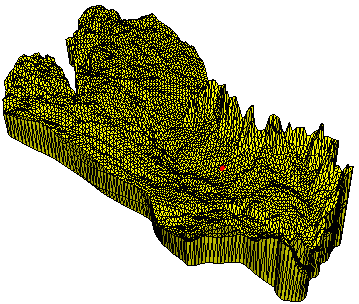
\includegraphics[width=0.3\linewidth]{colour-solid}\label{colour-solid}}\enspace
\subfloat[Default colour table]{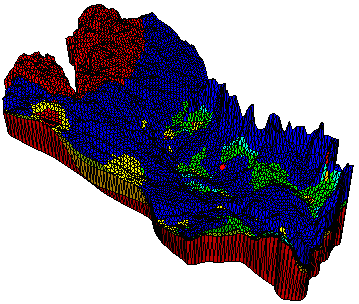
\includegraphics[width=0.3\linewidth]{colour-default}\label{colour-default}}\enspace
\subfloat[User-defined colours]{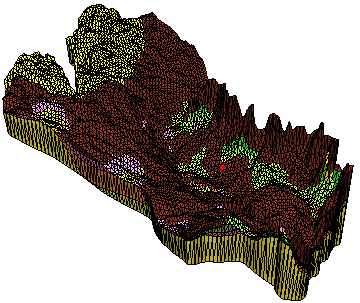
\includegraphics[width=0.3\linewidth]{colour-user}\label{colour-user}}
\end{center}
\caption{Each object is assigned a random solid colour as well as a default colour table based on a temperature scale (from blue to red). The solid colour can be adjusted via the ``Diffuse Color''-option (see section \ref{genvisoptions}), the colour table can be adjusted by loading a user-defined *.lut file via the ``Add color table...''-option (see section \ref{specvisoptions}).} \label{fig:colours}
\end{figure}

In detail these parameters are:

\begin{itemize}
\item Diffuse Color: Each item is assigned a colour which is used for rendering the object in 3D space. This colour can be changed here (see figure \ref{colour-solid}).
\item Active Scalar: Each visualisation object has an assigned colour which is used in the rendering process (see above). However, some data sets contain additional information (e.g. material groups for meshes, concentration of chemical substances, etc.). This information can be selected here and is then employed in the rendering of object in the render window (see figure \ref{colour-default}).
\item Visible Edges: Some objects (such as meshes) are composed of a combination of lines (edges) and surfaces. While the colour of the surfaces can be set using the \emph{Diffuse Color}-button, the colour of the edges can be changed here. Furthermore the rendering of edges can be switched off by unchecking the box next this option.
\item Opacity: Determines if an object appears to be transparent or not.
\item Scaling Factor: Super-elevates the data by the given factor. This makes it much more easy to recognise differences in height.
\end{itemize}

\section{Object-specific Visualisation Options}
\label{specvisoptions}

There are a number of options that are available only for certain types of data. These options can be selected by right-clicking on an item in the visualisation pipeline.

\begin{itemize}
\item \textbf{Add filter...:} Allows to apply a filter to the current objects. For details on that option see section \ref{filters}.
\item \textbf{Add color table...:} Allows you to assign a specific colour table to the currently selected scalar array. The colour table is loaded from a *.lut-file (see figure \ref{colour-user}).\\
    This option is available for all objects except image data.
\item \textbf{Convert to Mesh...:} Allows to convert an object of the VTK-data type ``Unstructured Grid'' to be converted into an \ogs mesh. Objects of that type are basically meshes that are contained in different data structure than ``normal'' \ogs meshes. Therefore, this specifically allows the conversion of imported VTK-files to \ogs meshes.\\
    This option is available for all objects of type ``VTK\_UN\-STRUCT\-URED\_GRID'' (i.e. all mesh objects).
\item \textbf{Convert Image to Mesh...:} Generates an \ogs mesh based on a given raster file. Specifically, the result is mesh built from rectangular equilateral triangle elements, with two triangles forming on square (this is basically a representation of the pixels of the raster file). If the raster file contains ``NoData''-values (e.g. raster files created with a Geographic Information System), these values are ignored. See figure \ref{Filter-Img4}.\\
    This options is only available for image data (i.e. raster files).
\item \textbf{Export to VTK:} All objects displayed the render window are technically VTK-objects. Choosing this option saves these objects in VTK-format to a file. They can then be used in any software supporting this format (e.g. Paraview\footnote{http://www.paraview.org/}).
\item \textbf{Export to OpenSG:} Converts objects into OpenSG format (*.osg). This is another open source graphics format. It is also the format used by the UFZ VisLab. Specifically, this also implies that \emph{anything} that can be visualised in \ogs can also be exported to OpenSG and be presented in the VisLab.
\end{itemize}

\section{Applying Filters for Visualisation}
\label{filters}

In contrast to the options detailed in the previous section, filters are a manipulation of the actual graphics object to enhance, reduce or deform certain aspects of these objects for imparting information that might not be superficial\footnote{One might argue that this definition also holds true for the assignment of specific color tables which is accessed via right-click on an object. This inconsistency originates in the data structures the objects are stored in and in defining an easy-to-use workflow for using this functionality.}.

To apply a filter, right-click on an object in the visualisation pipeline and select \cmd{Add filter...}. A dialog will pop up which lets you select one of a number of available filters. As before, filters will only be displayed for objects they can be applied to. However, this does not mean that it makes sense to apply any filter to any object where it can be applied. Also note, that it is possible (and sometimes useful) to apply filters to filters to extract certain information bit by bit.
%
\begin{figure}[tb]
\begin{center}
\subfloat[Raster data]{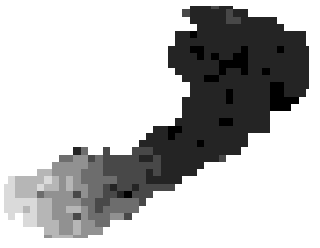
\includegraphics[width=0.4\linewidth]{Filter-Img1}\label{Filter-Img1}}\enspace
\subfloat[Apply lookup table to image]{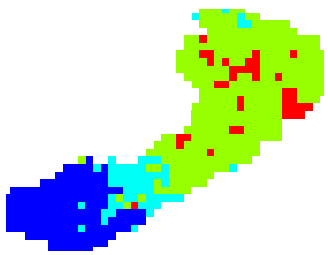
\includegraphics[width=0.4\linewidth]{Filter-Img2}\label{Filter-Img2}} \\
\subfloat[Image to bar chart]{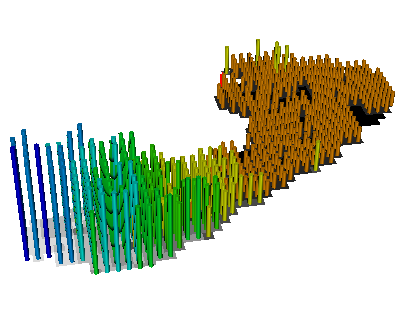
\includegraphics[width=0.4\linewidth]{Filter-Img3}\label{Filter-Img3}}\enspace
\subfloat[Convert Image to Mesh]{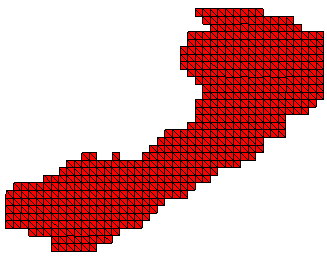
\includegraphics[width=0.4\linewidth]{Filter-Img4}\label{Filter-Img4}}
\end{center}
\caption{\ogs functionality applicable to image-/raster-data.} \label{fig:filter:raster}
\end{figure}
%
All available filters will be detailed in the following.

\subsubsection{Apply lookup table to image}
\bstart{Applicable to:} Image Data

\bstart{Effect:} Applies default color table to images, replacing grey values with a temperature scale (i.e. dark colours are blue, light colours are red). This results in an image where certain gradients are much better discernable. See figure \ref{Filter-Img2}.

\bstart{Remarks:} \emph{This is similar to applying a pre-defined colour table to a geometry- or mesh object. The implementation as a filter for images is based on the very different structure of image objects in the graphics library VTK which is used for visualisation.}

\begin{figure}[tb]
\begin{center}
\subfloat[Geometry Data]{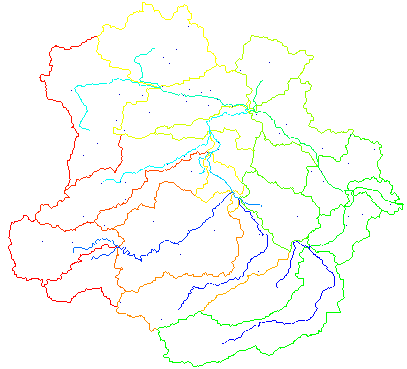
\includegraphics[width=0.4\linewidth]{Filter-Poly1}\label{Filter-Poly1}}\enspace
\subfloat[Points to Spheres]{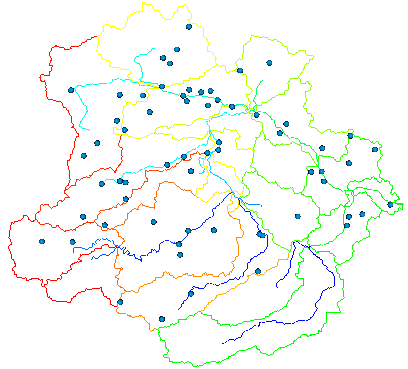
\includegraphics[width=0.4\linewidth]{Filter-Poly2}\label{Filter-Poly2}} \\
\subfloat[Lines to tubes]{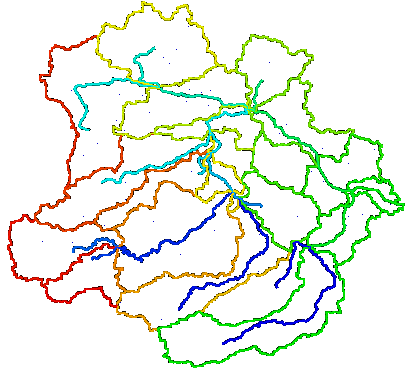
\includegraphics[width=0.4\linewidth]{Filter-Poly3}\label{Filter-Poly3}}\enspace
\subfloat[Extract cells by threshold]{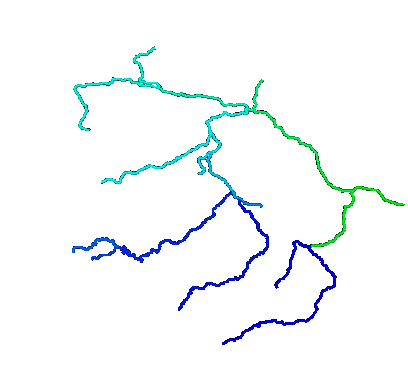
\includegraphics[width=0.4\linewidth]{Filter-Poly4}\label{Filter-Poly4}}
\end{center}
\caption{\ogs functionality applicable to geometry data. In figure \ref{Filter-Poly2} ground water stations in the area have been emphasised. In figure \ref{Filter-Poly4} a threshold filter has been applied to the tube-filtered data from figure \ref{Filter-Poly3} to select only the river network of the depicted area from the geometric data.} \label{fig:filter:poly}
\end{figure}

\subsubsection{Apply texture to surface}
\bstart{Applicable to:} Surfaces, Meshes

\bstart{Effect:} Allows to map an image/raster on a surface or mesh. This might be additional information such as land use classes, precipitation, etc. See figure \ref{Filter-Mesh4}.

\subsubsection{Elevation-based colouring}
\bstart{Applicable to:} Geometry, Meshes

\bstart{Effect: } Applies a colour to each point depending on the z-coordinate of that point, assuming that this denotes height in metres. The pre-defined colour scale starts with blue up to a height of $0$ metres (i.e. sea level), which is then slowly changing to green (150\,m) and yellow (450\,m) and then changing to red from then on. See figure \ref{Filter-Mesh2}.

\bstart{Remarks:} \emph{In theory these values can be changed. This is, however, currently not possible using the GUI.}

\begin{figure}[tb]
\begin{center}
\subfloat[Multilayered Mesh]{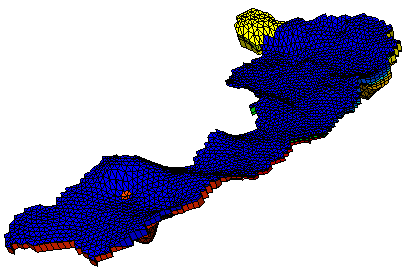
\includegraphics[width=0.4\linewidth]{Filter-Mesh1}\label{Filter-Mesh1}}\enspace
\subfloat[Elevation-based colouring]{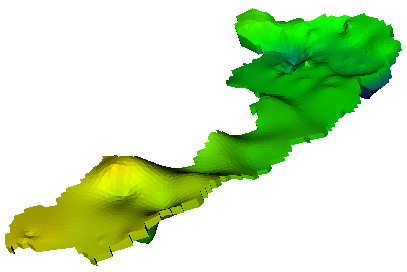
\includegraphics[width=0.4\linewidth]{Filter-Mesh2}\label{Filter-Mesh2}} \\
\subfloat[Extract cells by threshold]{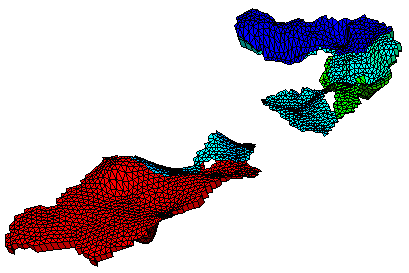
\includegraphics[width=0.4\linewidth]{Filter-Mesh3}\label{Filter-Mesh3}}\enspace
\subfloat[Apply texture to surface]{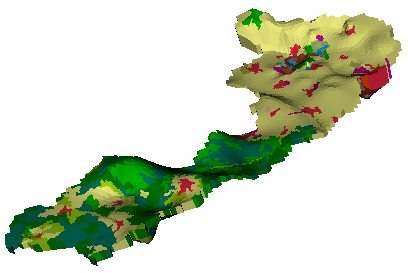
\includegraphics[width=0.4\linewidth]{Filter-Mesh4}\label{Filter-Mesh4}}
\end{center}
\caption{\ogs functionality applicable to meshes.} \label{fig:filter:mesh}
\end{figure}

\subsubsection{Extract cells by threshold}
\bstart{Applicable to:} Lines, Surfaces, Meshes

\bstart{Effect:} Each line, surface and mesh layer has a unique ID which allows to assign different colours to different objects. This filter furthermore allows to select a range of objects which should be displayed while all other objects are blanked out. This way you can visualise only a specified stratigraphic layer or a certain polyline, etc. See figures \ref{Filter-Poly4} and \ref{Filter-Mesh3}. The filter is always applied to the currently selected scalar array. For instance, given a mesh containing scalar arrays for material group and groundwater head, this filter may be used to select a range of materials (e.g. only materials with IDs 5--7) or regions with a certain groundwater head (e.g. $\text{head}>7.2$).

\subsubsection{Generate contours based on scalar fields}
\bstart{Applicable to:} Meshes

\bstart{Effect:} Given a scalar field this filter will output contour lines of meshes containing 2D elements and contour surfaces for meshes containing 3D elements. The number of contours that should be displayed can be defined in the filter properties as well as the minimum and maximum value for the calculated contours. The chosen number of contours will that be calculated on the selected scalar field in equidistant intervals between the chosen minimum and maximum value. The colours of the contours are automatically chosen based on these scalar values.

\subsubsection{Image to bar chart}
\bstart{Applicable to:} Image Data

\bstart{Effect:} Each pixel is assigned a bar depending on the grey value of the pixel. Also, the colour changes of that bar changes according to its height. See figure \ref{Filter-Img3}.

\bstart{Remarks:} \emph{This filter takes a lot of time for large images as the result becomes very complex. The intention is to use it for low resolution raster data of phenomena such as precipitation, etc.}

\emph{This is a good example on the combination of the successive application of these filters. This one combines `Image to vertical lines', `Lines to tubes' and `Elevation-based colouring'.}

\subsubsection{Image to vertical lines}
\bstart{Applicable to:} Image Data

\bstart{Effect:} Plots vertical lines for every pixel of a raster with each line having a height depending on the raster's grey value.

\bstart{Remarks:} \emph{This is a filter that is needed for the correct application of other filters. It is probably not of much use on itself.}

\subsubsection{Lines to tubes}
\bstart{Applicable to:} Geometry, Observation sites

\bstart{Effect:} A geometric line has independent of the current zoom level always a thickness of $1$. This filter allows to assign a `real' thickness to line-objects that also changes according to the current zoom. See figure \ref{Filter-Poly3}.

\subsubsection{Points to spheres}
\bstart{Applicable to:} Geometry, Observation sites

\bstart{Effect:} A geometric point has independent of the current zoom level always a diameter of $1$. This filter allows to assign a `real' diameter to point-objects that also changes according to the current zoom. See figure \ref{Filter-Poly2}.

\subsubsection{Surface filter}
\bstart{Applicable to:} Meshes

\bstart{Effect:} Extracts the outer surface of a mesh.

\bstart{Remarks:} \emph{This is a filter that is needed for the correct application of other filters. It is probably not of much use on itself.}
